\documentclass[letterpaper,12pt]{article}
\usepackage[T1]{fontenc}
\usepackage{mathptmx}

% unit definition
\usepackage{siunitx}
% \sisetup{load-configurations = abbreviations}
\DeclareSIUnit\inch{in}
\DeclareSIUnit\ft{ft}
\DeclareSIUnit\Rank{^{\circ} R}
\DeclareSIUnit\Faren{^{\circ} F}
\DeclareSIUnit\lbm{lb_{m}}
\DeclareSIUnit\lbf{lb_{f}}
\DeclareSIUnit\torr{Torr}
\DeclareSIUnit\gallon{gal}
\DeclareSIUnit\slug{slug}
\DeclareSIUnit\knots{kts}
\DeclareSIUnit\miles{mi}


% hyperlink formatting
\usepackage{hyperref}
\hypersetup{
    colorlinks=true,
    linkcolor=red,
    urlcolor=purple,
    citecolor=blue
}


% Other general packages
\usepackage{setspace}
\usepackage{graphicx}
\usepackage{float}
\usepackage{amsmath}
\usepackage{amssymb}
\usepackage{tabto}
\usepackage{booktabs, tabularx}
\usepackage{enumitem}
\usepackage{gensymb}
\usepackage{cancel}
\usepackage{tikz}
\usepackage{pgfplots}
\usepackage{appendix}
\usepackage[labelfont=bf, font={normalsize,stretch=1}]{caption}
\usepackage[letterpaper, margin=1.0in]{geometry}
\usepackage[utf8]{}
\usepackage{indentfirst}
\setlength{\parindent}{0.25in}

%Heading format
\usepackage{titlesec}
\titleformat*{\section}{\normalsize\bfseries}
\titleformat*{\subsection}{\normalsize\bfseries}
\titleformat*{\subsubsection}{\normalsize\bfseries}

%Page Numbers
\usepackage{fancyhdr} 
\pagestyle{fancy}
\fancyhf{}
\fancyheadoffset{0cm}
\renewcommand{\headrulewidth}{0pt} 
\renewcommand{\footrulewidth}{0pt}
\fancyhead[R]{\thepage}
\pagenumbering{arabic}

%listings package for code
\usepackage{listings}
\usepackage{xcolor}

% bibliography formatting
\usepackage{etoolbox}
\patchcmd{\thebibliography}{\section*{\refname}}{}{}{}
\setstretch{2}

% color definitions
\definecolor{dblue}{HTML}{145680}
\definecolor{dred}{HTML}{801414}
\definecolor{dgreen}{HTML}{148014}
\definecolor{bgcode}{rgb}{0.95,0.95,0.95}
\definecolor{codegreen}{rgb}{0,0.6,0}
\definecolor{codegray}{rgb}{0.5,0.5,0.5}
\definecolor{codepurple}{rgb}{0.58,0,0.82}
\definecolor{backcolour}{rgb}{0.95,0.95,0.92}

\lstdefinestyle{mystyle}{
    backgroundcolor=\color{backcolour},
    commentstyle=\color{codegreen},
    keywordstyle=\color{magenta},
    numberstyle=\tiny\color{codegray},
    stringstyle=\color{codepurple},
    basicstyle=\ttfamily\footnotesize,
    breakatwhitespace=false,
    breaklines=true,
    captionpos=b,
    keepspaces=true,
    numbers=left,
    numbersep=5pt,
    showspaces=false,
    showstringspaces=false,
    showtabs=false,
    tabsize=2
}
\lstset{style=mystyle}

\pgfplotsset{compat=1.17}

% NOTES
%  - Double spacing (always fix for figures and tables though)
%  - for tables, remember to make them single spaced using \renewcommand{\arraystretch}{1}
%  - Always pull from GitHub to Overleaf when there are commits to be pulled (Menu > GitHub > PULL)
%  - for REFERENCES, use \cite{<label>} to link the reference.

% % TABLE TEMPLATE
% \begin{table}[H]
%     \begin{center}
%     \setstretch{1} 
%     \caption{\textbf{<caption here>}} \label{table:<label here>}
%     \begin{tabular}{|p{0.3in}|p{1in}|p{1in}|} % set column nums and width
%         \hline \textbf{No.} & \textbf{Item} & \textbf{Weight} \\ \hline % column headers
%         1 & Hot dogs & 2 lbs \\ \hline
%     \end{tabular}
%     \end{center}
% \end{table}

\begin{document}

%%% Title Pa
\begin{center}
    {\Large\textbf{AE 484 Homework 4}}\\
    Anshuk Chigullapalli, Max Kaiser, George Petrov, Kenneth Tochihara, Jeffery Zhou\\
\end{center}

% George, Anshuk, Kenneth
\section{Vehicle Design}

    % Anshuk
    \subsection{Fabrication Drawings}
    % Detail 3 view drawings (or two views when appropriate) view drawings of all fabricated components sufficiently dimensioned for manufacturing. Note that complex curves such as airfoils can show overall dimensions (like the chord length and thickness) with a leader and note to the surface indicating that the curve will be provided electronically. Be sure to name all parts and indicate the quantity and material they are made out of.
    
    The fabricated components of the aircraft include the  wings (and the cutouts in their foam), the vial release mechanism, the spars and the winglets. Some of these components have complex geometries that will require the use of computer aided manufacturing such as 3D printing or CNC machining. The engineering drawings for all the relevant components are provided in the Appendix.
    
    % insert images of the dimensioned drawings? Or create an appendix
    
    % add a table of all the fabricated parts
    
     \begin{table}[H]
         \begin{center}
         \caption{\textbf{Fabricated Components}} \label{table:fab_components}
         \begin{tabular}{|p{2in}|p{1in}|p{1in}|p{1in}|} % set column nums and width
             \hline \textbf{Component} & \textbf{Quantity} & \textbf{Material} & \textbf{Comments} \\ \hline % column headers
             Wing & 2 & Foam & bruh \\ \hline
         \end{tabular}
         \end{center}
     \end{table}
    
    % Anshuk
    \subsection{Full Assembly}
    % A fully assembled drawing showing the locations of all the parts and overall dimensions of key elements of the aircraft when it is put together. This should be presented both as a 3 view and isometric view drawing with all the parts named on the drawing.
    
    The team assembled all the individual components together in Siemens NX and created the full aircraft engineering drawing, provided in the Appendix. The overall dimensions are provided in the table below.
    
    
    % Create a table with the overall dimensions
    
    
    % Kenneth
    \subsection{Equipment Locations}
    % A fully assembled drawing showing the locations of the equipment and instrumentation (components you buy and don’t fabricate like the receiver, servos, motor, battery, camera, video transmitter, ESC, etc.) on or within the airframe with key dimensions given for placement. This should be presented both as a 3 view and isometric view drawing and it may be useful to use cut-away views in some cases to better show where equipment/components are located.
    
        % 1. Reciever
        % 2. Vial Servo
        % 3. Motor
        % 4. Battery
        % 5. ESC
        % 6. +Y Elevon Servo
        % 7. -Y Elevon Servo
    \begin{table}[H]
    \begin{center}
    \caption{\textbf{Component Locations}} \label{tab:component_locations}
    \begin{tabular}{|c|c|} 
        \hline
        \textbf{No.} & \textbf{Component} \\ \hline
        1 & Reciever \\ \hline
        2 & Vial Servo \\ \hline
        3 & Motor \\ \hline
        4 & Battery \\ \hline
        5 & ESC \\ \hline
        6 & +Y Elevon Servo \\ \hline
        7 & -Y Elevon Servo \\ \hline
    \end{tabular}
    \end{center}
    \end{table}
    
    % George
    \subsection{Exploded View}
    % An isometric exploded view assembly drawing with all the fabricated parts and purchased components labeled. No dimensions are needed for this drawing.\
    Below, an exploded view render of all the components can be seen. Appendix \ref{ApxB}, shows the full engineering drawing of the render below.
        \begin{figure}[H]
            \centering
            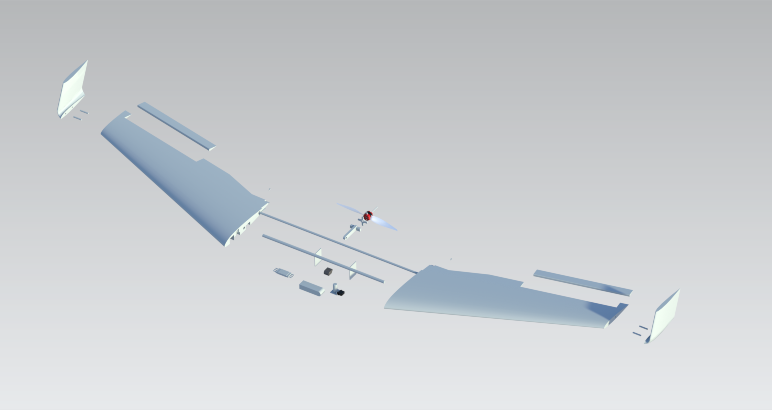
\includegraphics[width=0.8\textwidth]{homeworks/homework4/report/Figure/aircraft_assembly_exploded.png}
            \caption{\textbf{Aircraft Exploded View}}
            \label{fig:exploded}
        \end{figure}
    
    % Theses drawings will be graded on how well and detailed you present your design. Include table of the characteristics of the tail and wing (airfoils, aerodynamic centers, S, MAC, sweep, taper, root chord, tip cord, twist, tail length etc.).
    
    % Kenneth
    \subsection{Design Overview}
    % Write a brief paragraph describing your design and the drawings presented.
    
        The aircraft was designed as a flying wing with tall winglets to add yaw stability to the flight. These winglets are secured with epoxied dowels to firmly secure the two components together. The main wing is assembled onto two carbon fiber spars. These lengths were determined based on the available at the source provided for carbon fiber tube purchases. Many of the components were mounted into the wing underneath to reduce protrusions throughout the body of the aircraft. Holes for servos, receiver, motor mount, battery, and vial mechanism all have cutouts to mount these components inside. Control surfaces and their actuators were included in the design to further increase the fidelity of model. A preliminary design of the hand holder was also included, with plans to refine the model in the future to incorporate throwing mechanics and ergonomics.

% Anshuk    
\section{Vial Release Mechanism}
% Using figures and sentences/paragraphs describe your mechanism to release the protective vial described in the problem statement (cylinder 0.75” in diameter, 1.5” long and a mass of 5 grams) and how it works. What are the benefits and possible concerns you have with your design?

    The team decided to use a vial mechanism that was simple in design with minimal use of heavy parts or complex actuator mechanisms. The design was also kept within a size constraint so that the design would fit in front of the spars, helping keep the Center of Gravity in front of the Center of Pressure. 
    
    The design includes a 3D-printed plate that is connected to a servo arm placed next to the plate. The plate acts as a trap door at the bottom of the aircraft.The vial is placed on the flat plate in an upright position. When the servo actuates, the flat plate rotates with it away from the bottom and creates an opening out of the plane. The vial then falls out of the plane to be caught by someone on the ground.
    
    Figure \ref{fig:vial_assembly} shows the vial release mechanism assembly on its own and Figures \ref{fig:vial_closed} and \ref{fig:vial_open} shows the vial release assembly on the underside of the wing in the aircraft in both the open and closed configurations respectively.
    
    \begin{figure}[H]
        \centering
        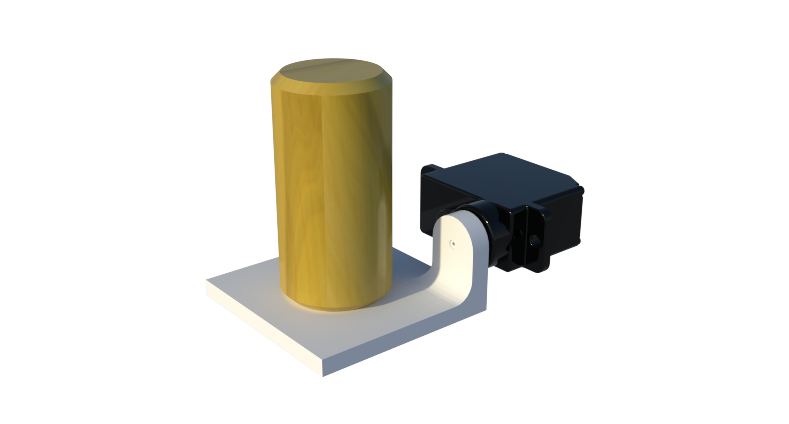
\includegraphics[width=0.65\textwidth]{homeworks/homework4/report/Figure/assembly_vial_door.png}
        \caption{\textbf{Vial Release Mechanism}}
        \label{fig:vial_assembly}
    \end{figure}
            
    \begin{figure}[H]
        \centering
        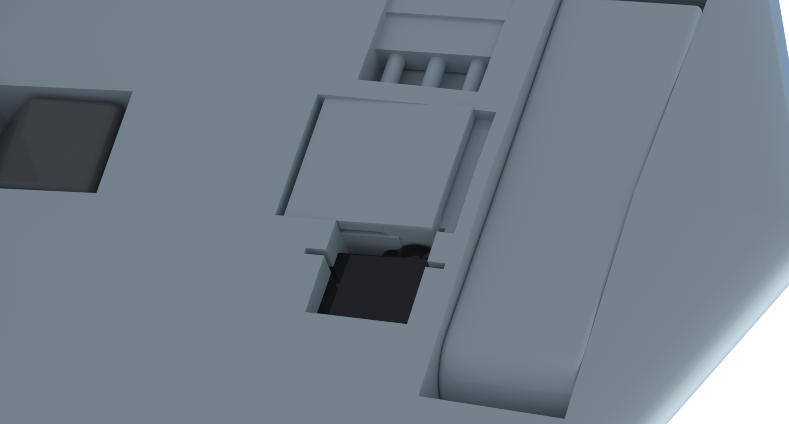
\includegraphics[width=0.55\textwidth]{homeworks/homework4/report/Figure/aircraft_assembly_door_closed.png}
        \caption{\textbf{Vial Mechanism in the Closed Configuration}}
        \label{fig:vial_closed}
    \end{figure}
    
    \begin{figure}[H]
        \centering
        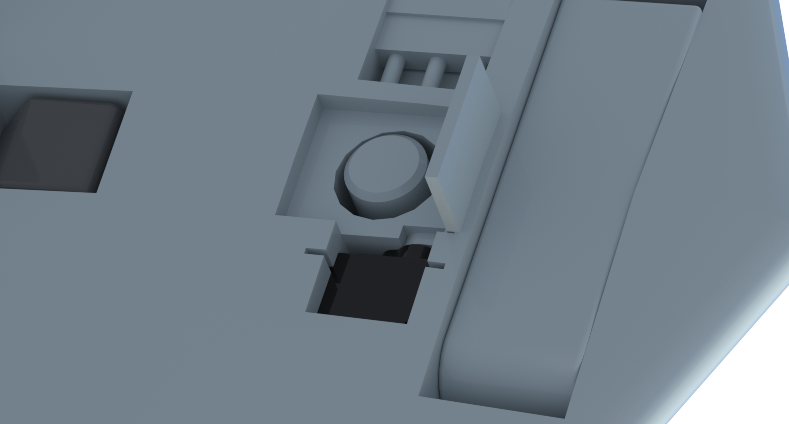
\includegraphics[width=0.55\textwidth]{homeworks/homework4/report/Figure/aircraft_assembly_door_open.png}
        \caption{\textbf{Vial Mechanism in the Open Configuration}}
        \label{fig:vial_open}
    \end{figure}
    
    This design involves only one moving part connected to the servo, and so was chosen for its simplicity and ease of building. The only harnessing required in this design would be for the servo, because the plate is attached to the servo itself and the vial sits freely. The primary concern is ensuring that we cut the foam around the mechanism in the right way to account for the rotation of the flat plate. The team plans on fixing this concern by making the CAD accurate and fixing any tolerance issues so we can cut the fuselage foam accordingly.
    
% Jeff
\section{Free-Body Diagram}
% Using the weights and positions of all components (i.e. instrumentation, servos, motor, battery etc.) draw a free body diagram (using the CAD package) and calculate a force and moment balance using an appropriate reference point. Calculate the center of gravity of all the fabricated parts and components and list their coordinates relative to an appropriate reference point. Calculate the weight and center of gravity of the entire vehicle and write a short paragraph describing your analysis.

% Jeff
\section{Prominent Forces}
% Based on your drawing write a short description indicating how the major forces and moments (i.e. weights, aerodynamic forces/moments, thrust etc.) will be structurally supported by your airframe design. Feel free to use neat simplified sketches and analysis to indicate how the stresses are carried by the airframe structure. Indicate the major regions of where stress concentrations may be the largest concern in your design.

% Max
\section{Design Characteristics}
% Provide tables of the characteristics [dimensions, airfoils, planform area, span, chord lengths, dihedral (if any), taper ratio, sweep, mean aerodynamic chord, root and mean chord length, elevon size (span and % chord), aerodynamic center and winglet or vertical stabilizer size (chord lengths, taper ratio etc.). write a short paragraph or two describing the process you used to determine the size and shape of the wing, elevons, and winglets. Justify why the wing elevons and winglets are the size and shape you have described. Also justify why you selected the airfoils that you are using.

    \begin{center}
    \begin{tabular}{|c|c|} 
        \hline
        \textbf{Characteristic} & \textbf{Value} \\ \hline
        Wingspan (in) & 69.5 \\ \hline
        Length (in) & 22.07 \\ \hline
        Airfoil & NACA 23012 \\ \hline
        Planform Area (in$^2$) & 748 \\ \hline
        Root Chord Length (in) & 14.5 \\ \hline
        Tip Chord Length (in) & 7.5 \\ \hline
        Taper Ratio & 6.182 \\ \hline
        Sweep (deg) & 22.019 \\ \hline
        Mean Aerodynamic Chord (in) &  11.371 \\ \hline
        Aerodynamic Center (in) & 9.635 \\ \hline
        Elevon Span (in) & 17 \\ \hline
        Elevon Chord Percentage (\%) & 20 \\ \hline
        Winglet Area (in$^2$) & 30 \\ \hline
        Winglet Airfoil & NACA 0010 \\
        \hline
    \end{tabular}
    \end{center}

    We decided the size and shape of the wing based on a few factors. The first choice we made was in the wing span as we wanted to have the widest wings allowable to produce the most effective lift we could with our design. We then decided we wanted at least 20 deg of sweep in our wing to ensure that we had adequate yaw stability without having to include massive winglets in our design. Having these two quantities specified, we chose the airfoil in concert with choosing the root chord length of our plane, as we wanted to use the entire thickness allotted so that we would be able to fit a majority of the components within the wing and without the need for an additional fuselage. We chose the NACA 23012 airfoil because we wanted an airfoil with 1-2 deg of chamber and this airfoil looked like it would give us a large internal volume for our internal components. The mean chord length was chosen based on the thickness of the NACA 23012 so give us 1.75 inches of thickness. We also found in testing that the NACA 23012 also has a center of pressure that is farther back that other airfoils we tested, proving useful with our pusher motor configuration and subsequent COG. The tip chord length was set at 7.5 to give us sufficient room to attach adequately sized winglets. 

    After having chosen our wing design, we moved on to designing the winglets of our UAV. Since we had already determined a sweep over 20 deg we did not need to create large winglets. We decided on an area of 30 $\text{in}^2$ to generate some more lateral stability without adding too much weight to the ends of our wings. As for the elevons, we wanted to incorporate about 50\% of the wingspan, set to the outside for increased leverage about the center line of our design. We also saw literature that suggested at least $\frac{1}{8}$ of the chord length to be taken up by the elevon, so we went with 15\% to ensure we have enough area to effectively control our UAV.


% Max
\section{Flight Characteristics}
% Write a paragraph and present calculations/analysis Indicating why your CG is located appropriately to achieve stability. Hint: Evaluate the longitudinal static margin of your simplified aircraft (i.e. wing without the winglets or vertical stabilizer) using XFLR5 and locating the neutral point. Also give conceptual arguments of the aircrafts lateral and directional stability. In addition to where you have placed the battery show that it can be adjusted along the axis (i.e. if possible it is good to allow the battery to be placed over the quarter chord (MAC) location on the wing). Provide a table of the overall geometric and flight characteristics of your aircraft (neutral point, SM, design α, design velocity, overall weight, etc.) and your best estimate velocity and angle of attack when hand launched. From your analysis provide graphs of (CD, CL, CL/CD, CM, vs. α) and describe their characteristics and what you conclude from them. Be sure to include paragraphs describing these results as they are presented and justifying your decisions.

% Max
\section{Mass Estimates}
% Calculate the total weight of your aircraft (including the battery, motor, and vial delivery system) and describe how you determined it. What is the power to weight ratio and wing loading of your aircraft? Write a paragraph describing your analysis.

    \begin{center}
    \begin{tabular}{|c|c|} 
    \hline
        \textbf{Component} & \textbf{Weight (g)} \\ \hline
        Main Wings & 710 \\ \hline
        Winglets & 66 \\ \hline
        All equipment & 581 \\ \hline
        \textbf{Total Weight} & \textbf{1357} \\ \hline
    \end{tabular}
    \end{center}

    We went about calculating the weight using the features XFLR5 provides for weighting. We estimated the mass of the wings and winglets by using the wing area feature and the weight per unit area measurements provided in the lecture notes. Once we had these figures we were able to move on to the point masses in our aircraft which represent all the components and bracing that we are going to put into it. These were added in XFLR5 with placement as according to our CAD model, with the weights being figures taken either directly from course material or from the website with the listings of the carbon fiber tubes that we will use for the spars. We then added about 45 grams of additional weight that would account for any extra material we would use to connect our components back into the main spars. Given the wings, winglets, all equipment and extra weight we came in at about 0.02 pounds under our 3 pound limit. 
    
    The wing loading of our UAV is about 2 g/in$^2$, which was determined using the wing loading feature given in XFLR5. The power to weight ratio is a little harder to determine. We went to an R/C hobby website where there was a power vs. voltage and amperage table. For this determination we will assume that the battery will be outputting 11.1V and 24 amps. With these values our motor will be outputting 266.4 watts. Using this power and our weight of 1,357 grams we were able to determine that our UAV will have a power to weight ratio of 5.09 g/W.

\appendix
\renewcommand{\thesection}{\textbf{Appendix \Alph{section}:}}

\section{Sample Calcs} \label{apx:sample_calc}
\begin{enumerate}[wide,label=\textbf{\arabic*}., labelindent=0pt]

    \item \textbf{Wing Loading}
        \[W/S = \frac{W}{S_{ref}}\]
        $ W =$ weight [oz]\\
        $S_{ref} =$ wing reference area [ft$^2$]\\
        
        \begin{align*}
            W/S &= \frac{47.867}{16985}\\
            &= 9.18 \text{ oz/ft$^2$}\\
        \end{align*}
        
        \item \textbf{Aspect Ratio}
        \[AR = \frac{b^2}{S_{ref}}\]
        $ b =$ span [in]\\
        $S_{ref} =$ wing reference area [in$^2$]\\
        
        \begin{align*}
            AR &= \frac{69.8^2}{746.330}\\
            &= 6.530 \text{ N.D.}\\
        \end{align*}
    
    \item \textbf{Center of Gravity}
        \[C_g = \frac{\sum_i m_i x_i }{\sum_i m_i}\]
        $ m =$ mass [g]\\
        $ x =$ distance from tip in x-direction [in]\\
        
        \begin{align*}
            C_g &= \frac{47.867}{16985}\\
            &= \color{red}{JEFFFFFFFFFFFFFFFFFFFFF}9.18 \text{ g/in$^2$}\\
        \end{align*}
        
    \item \textbf{Taper Ratio}
        \[\lambda = \frac{c_t}{c_r}\]
        $ c_t =$ tip chord [in]\\
        $ c_r =$ root chord [in]\\
        
        \begin{align*}
            \lambda &= \frac{7.5}{14.5}\\
            &= 0.517 \text{ N.D.}\\
        \end{align*}    
 
\section{Engineering Drawings} \label{apx:eng_drawings}
    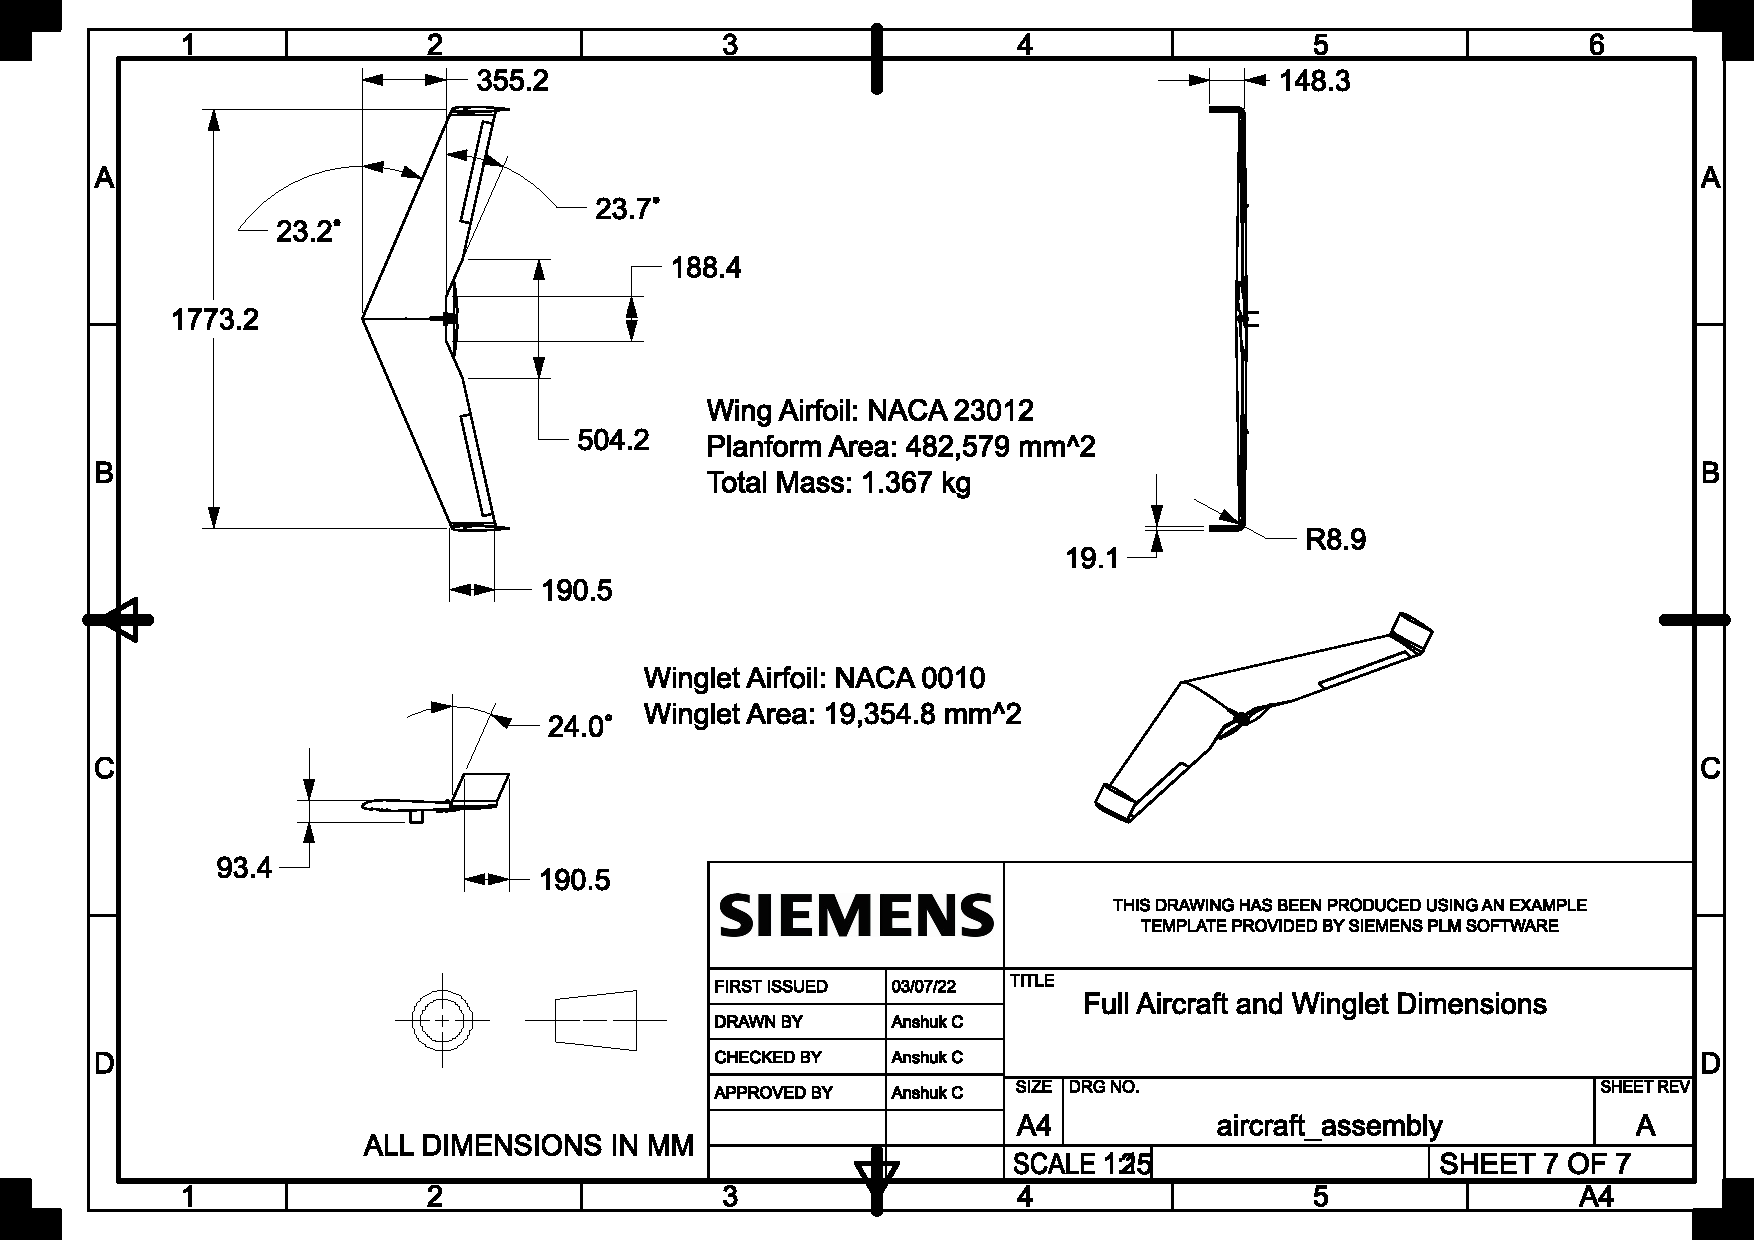
\includepdf[pages=-,angle=90]{homeworks/homework4/report/Figure/anshukc2_aircraft_dimensions.pdf}
    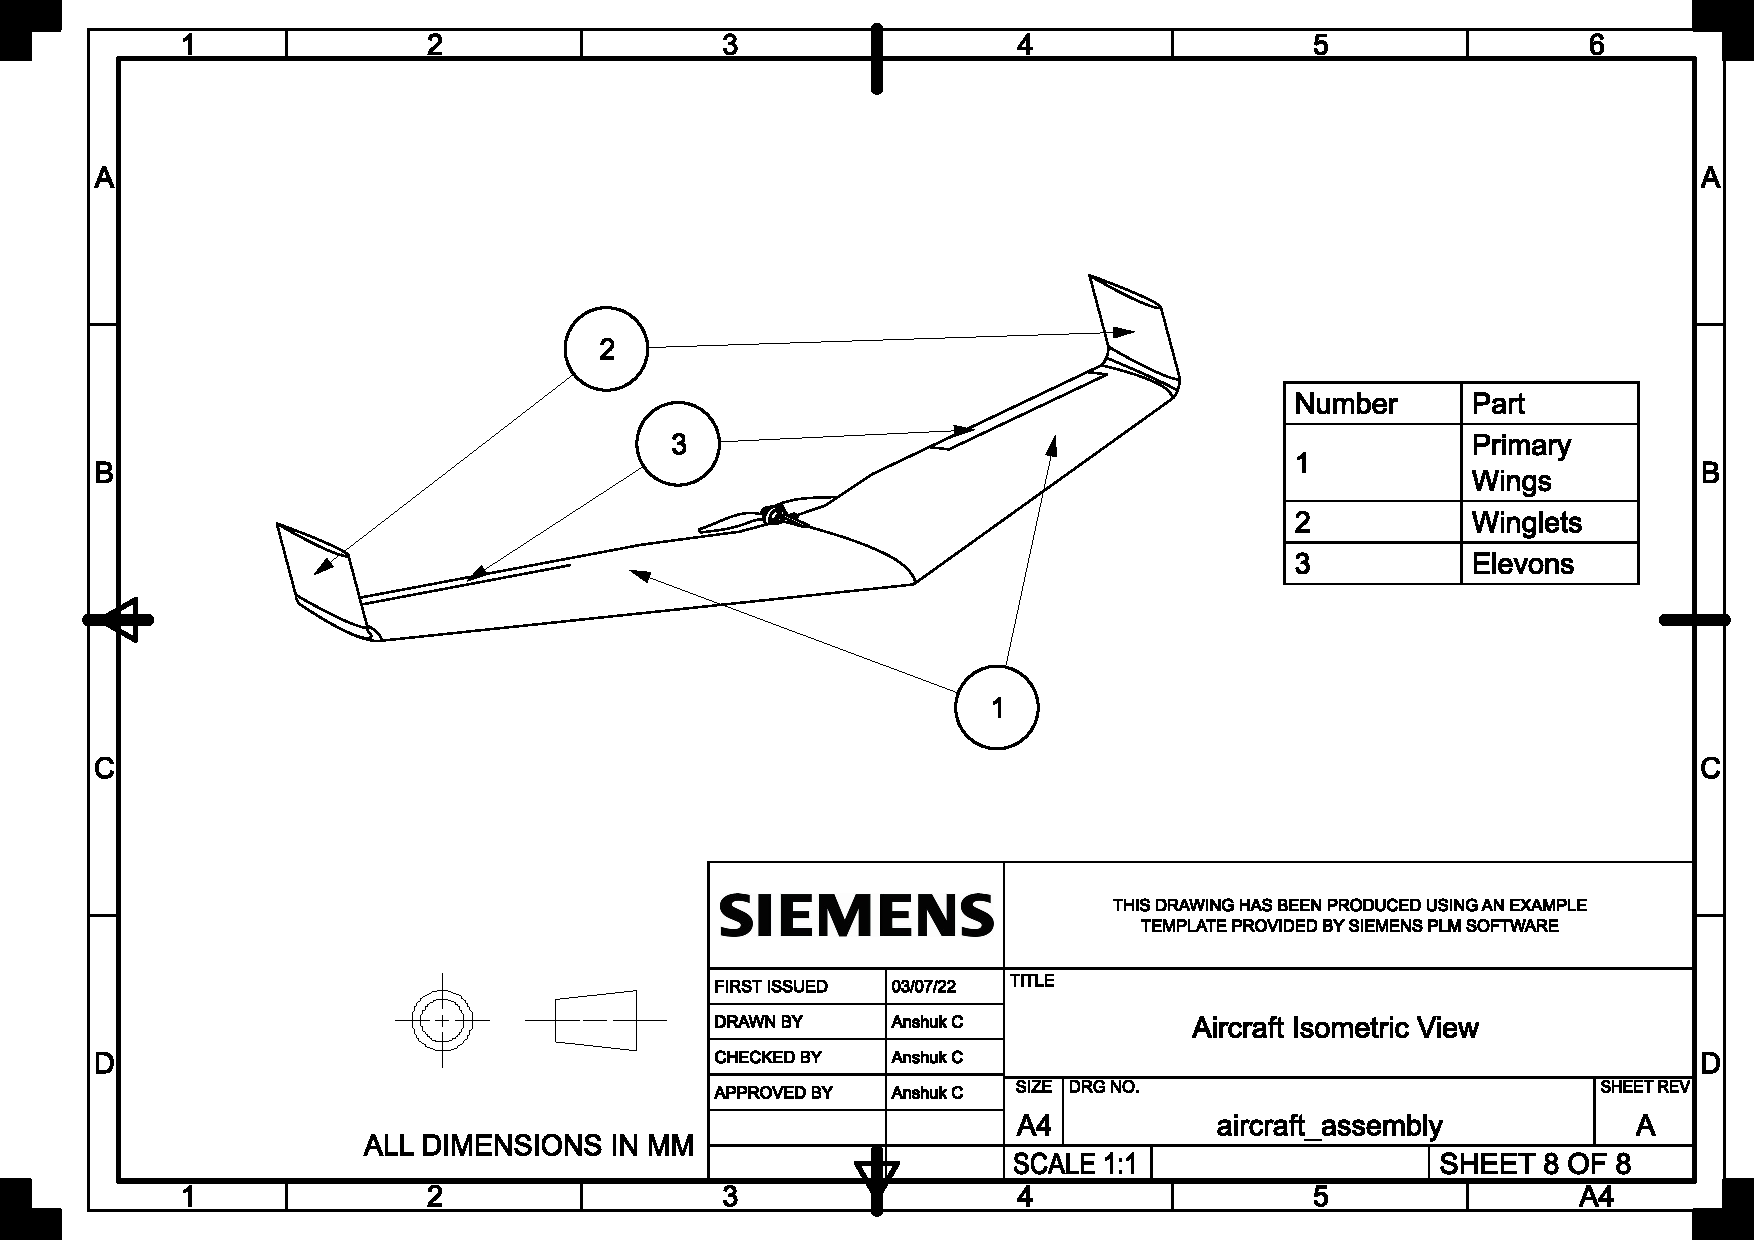
\includepdf[pages=-,angle=90]{homeworks/homework4/report/Figure/anshukc2_aircraft_isometric_drawing.pdf}
    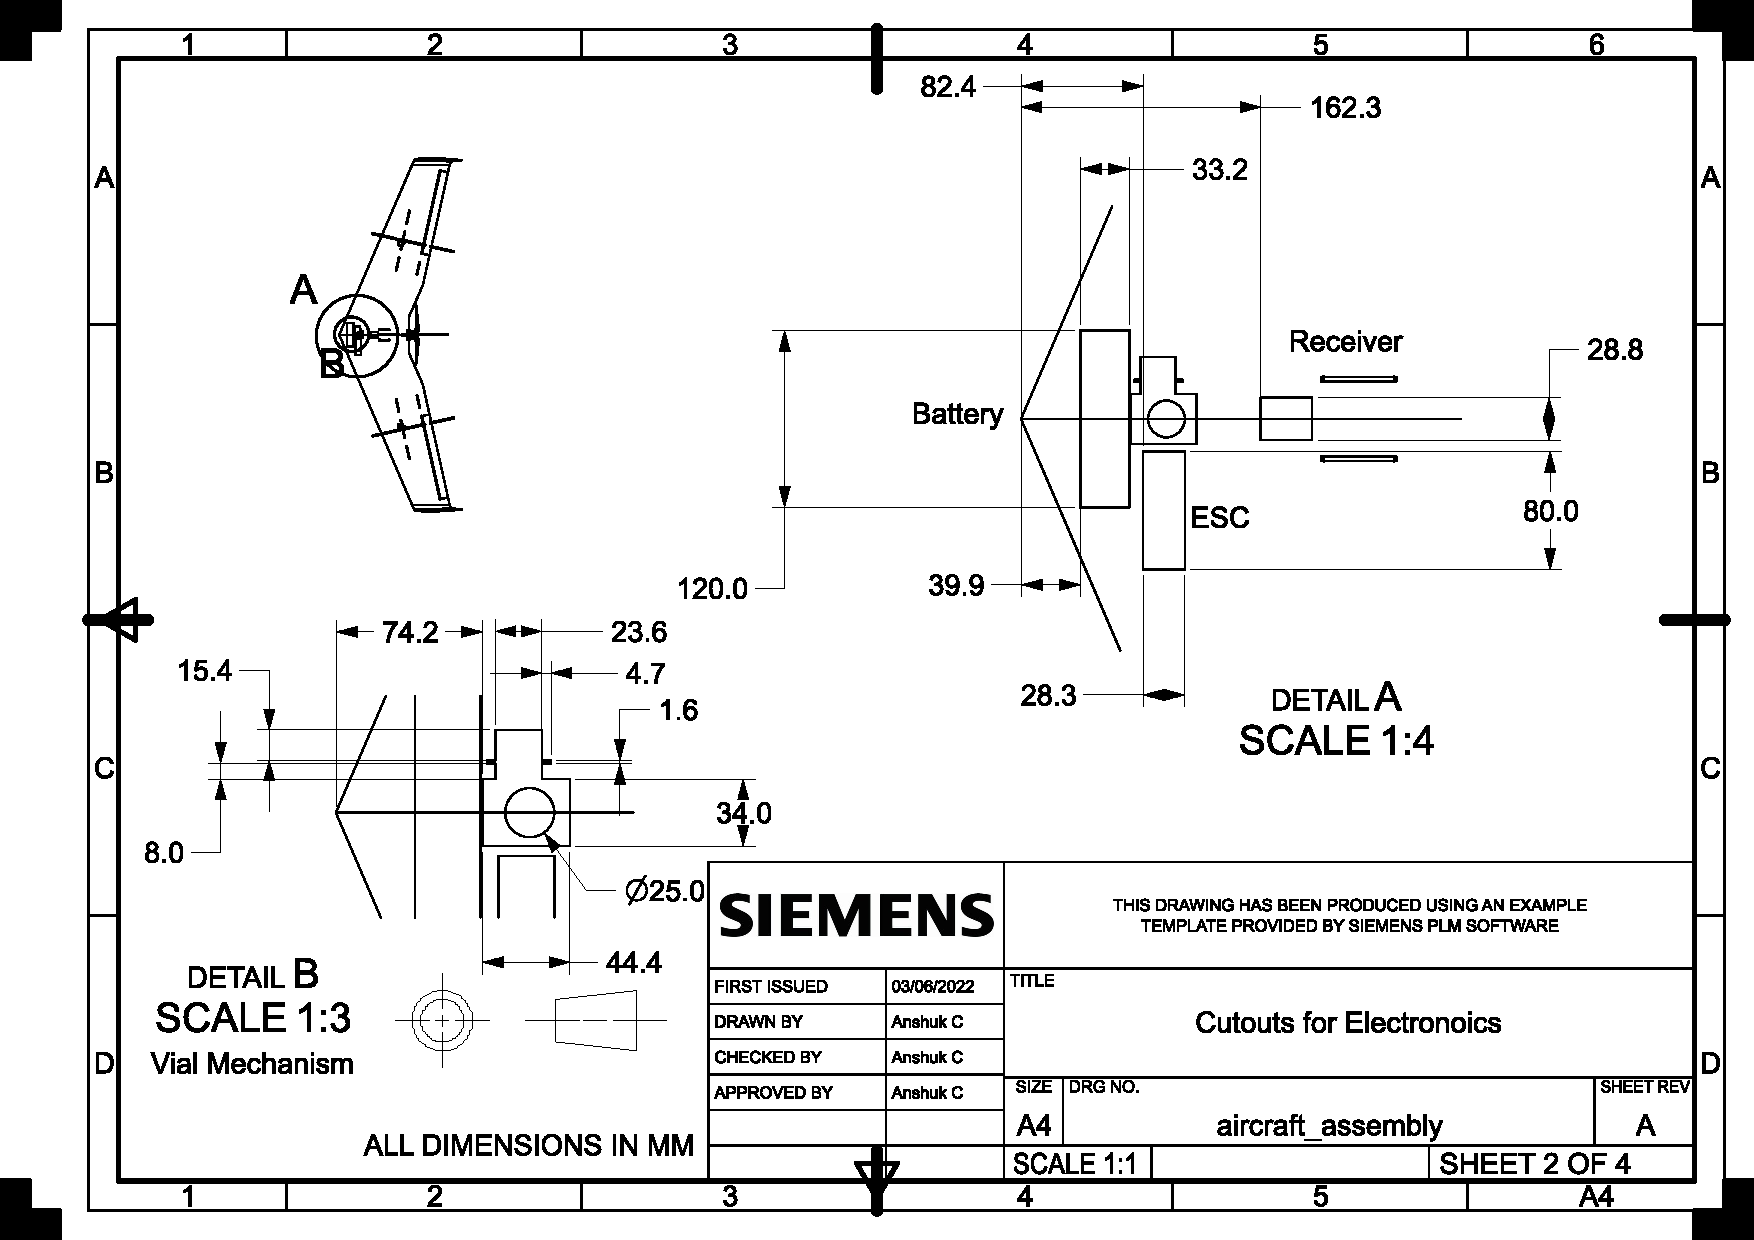
\includepdf[pages=-,angle=90]{homeworks/homework4/report/Figure/electronics_cutouts.pdf}
    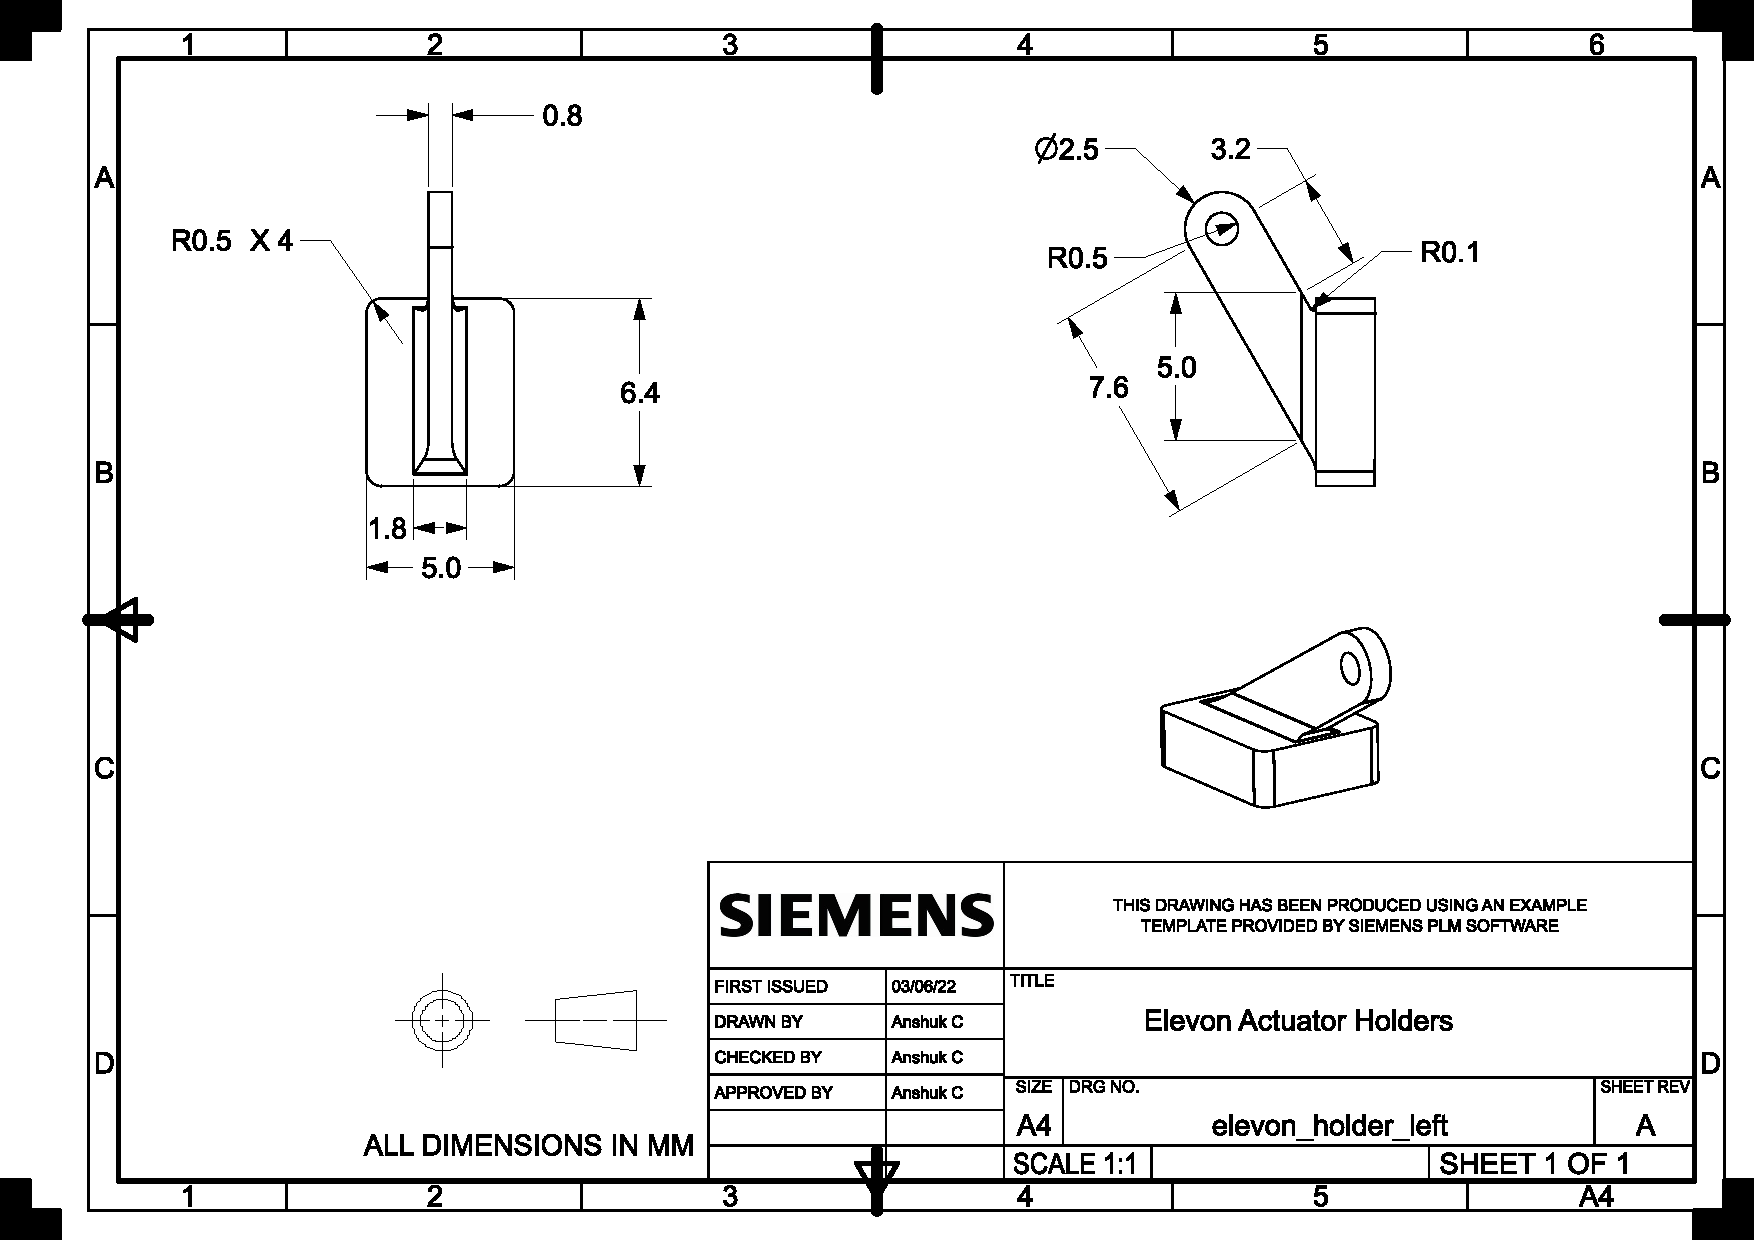
\includepdf[pages=-,angle=90]{homeworks/homework4/report/Figure/elevon_holders.pdf}
    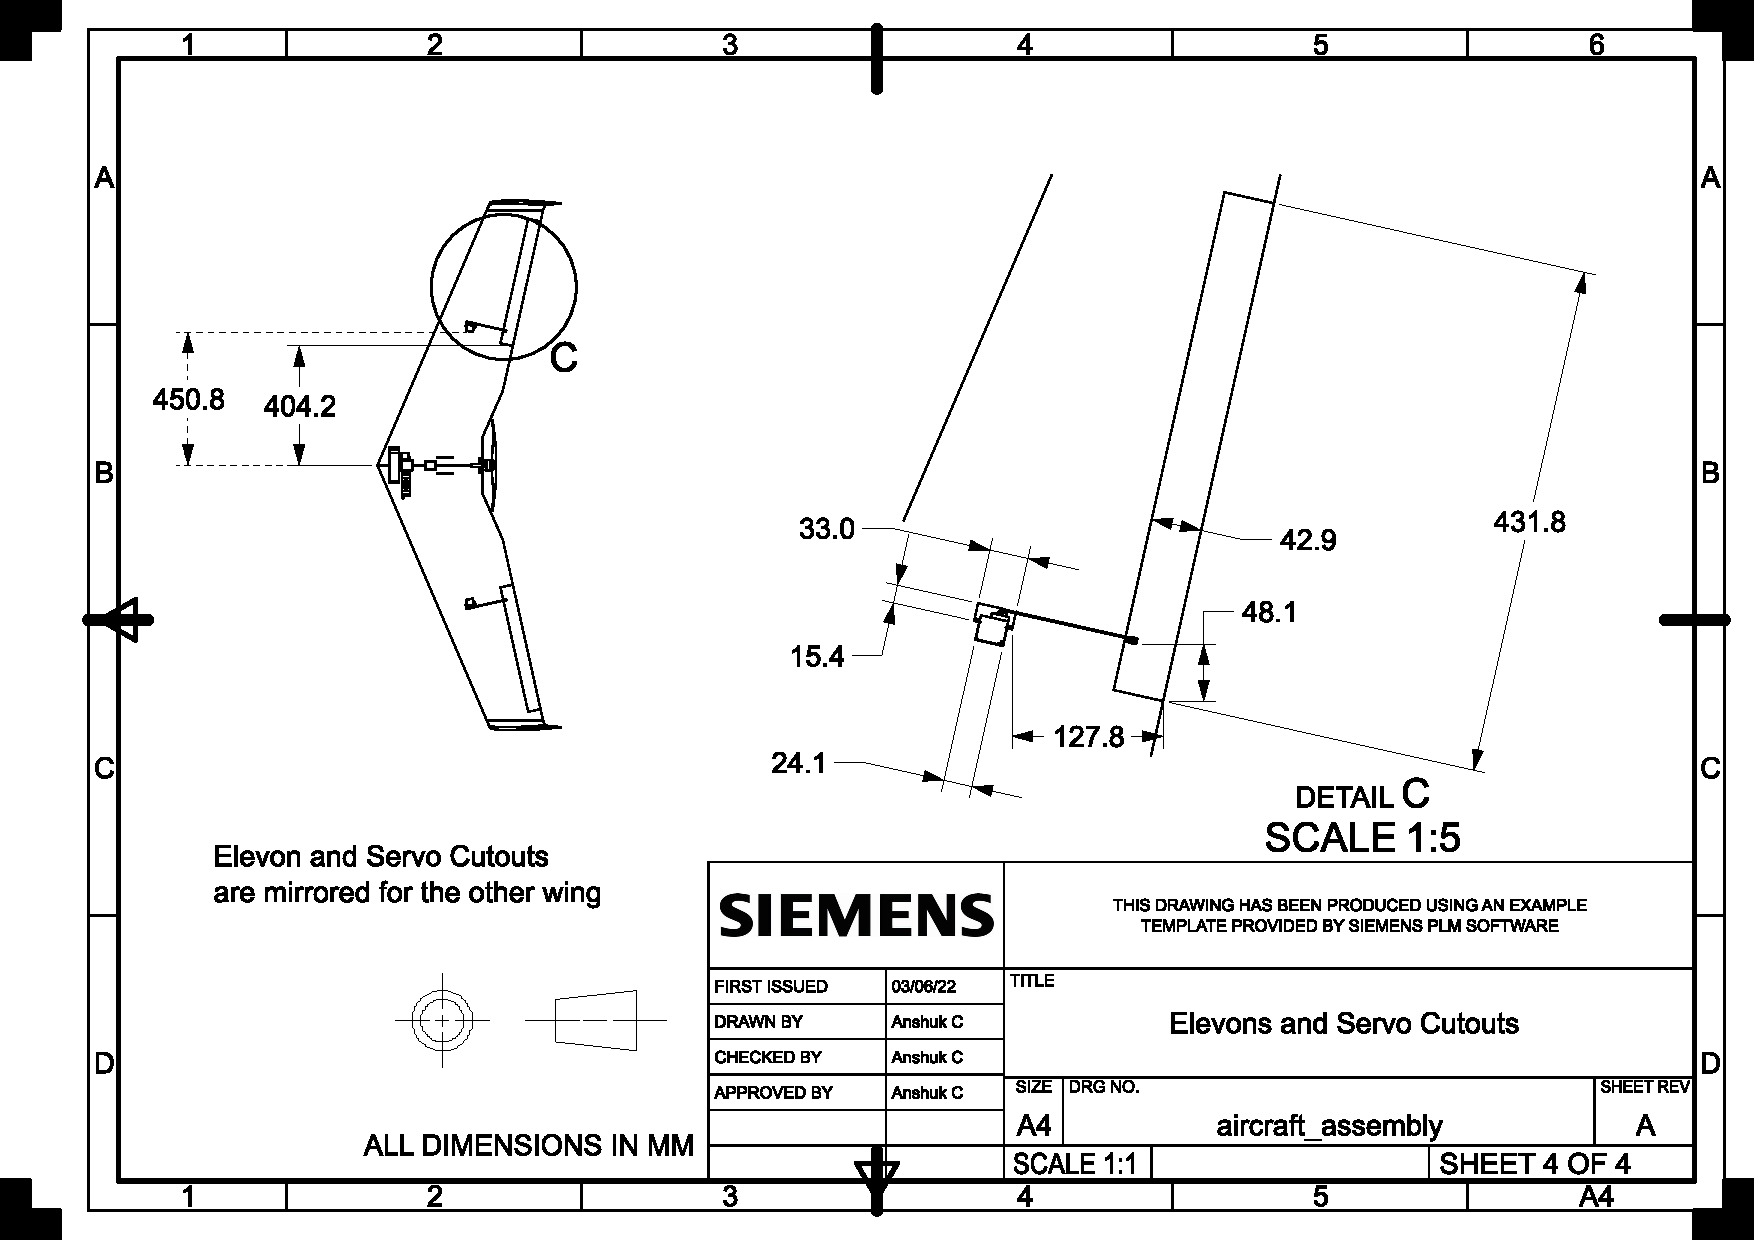
\includepdf[pages=-,angle=90]{homeworks/homework4/report/Figure/elevons_servos.pdf}
    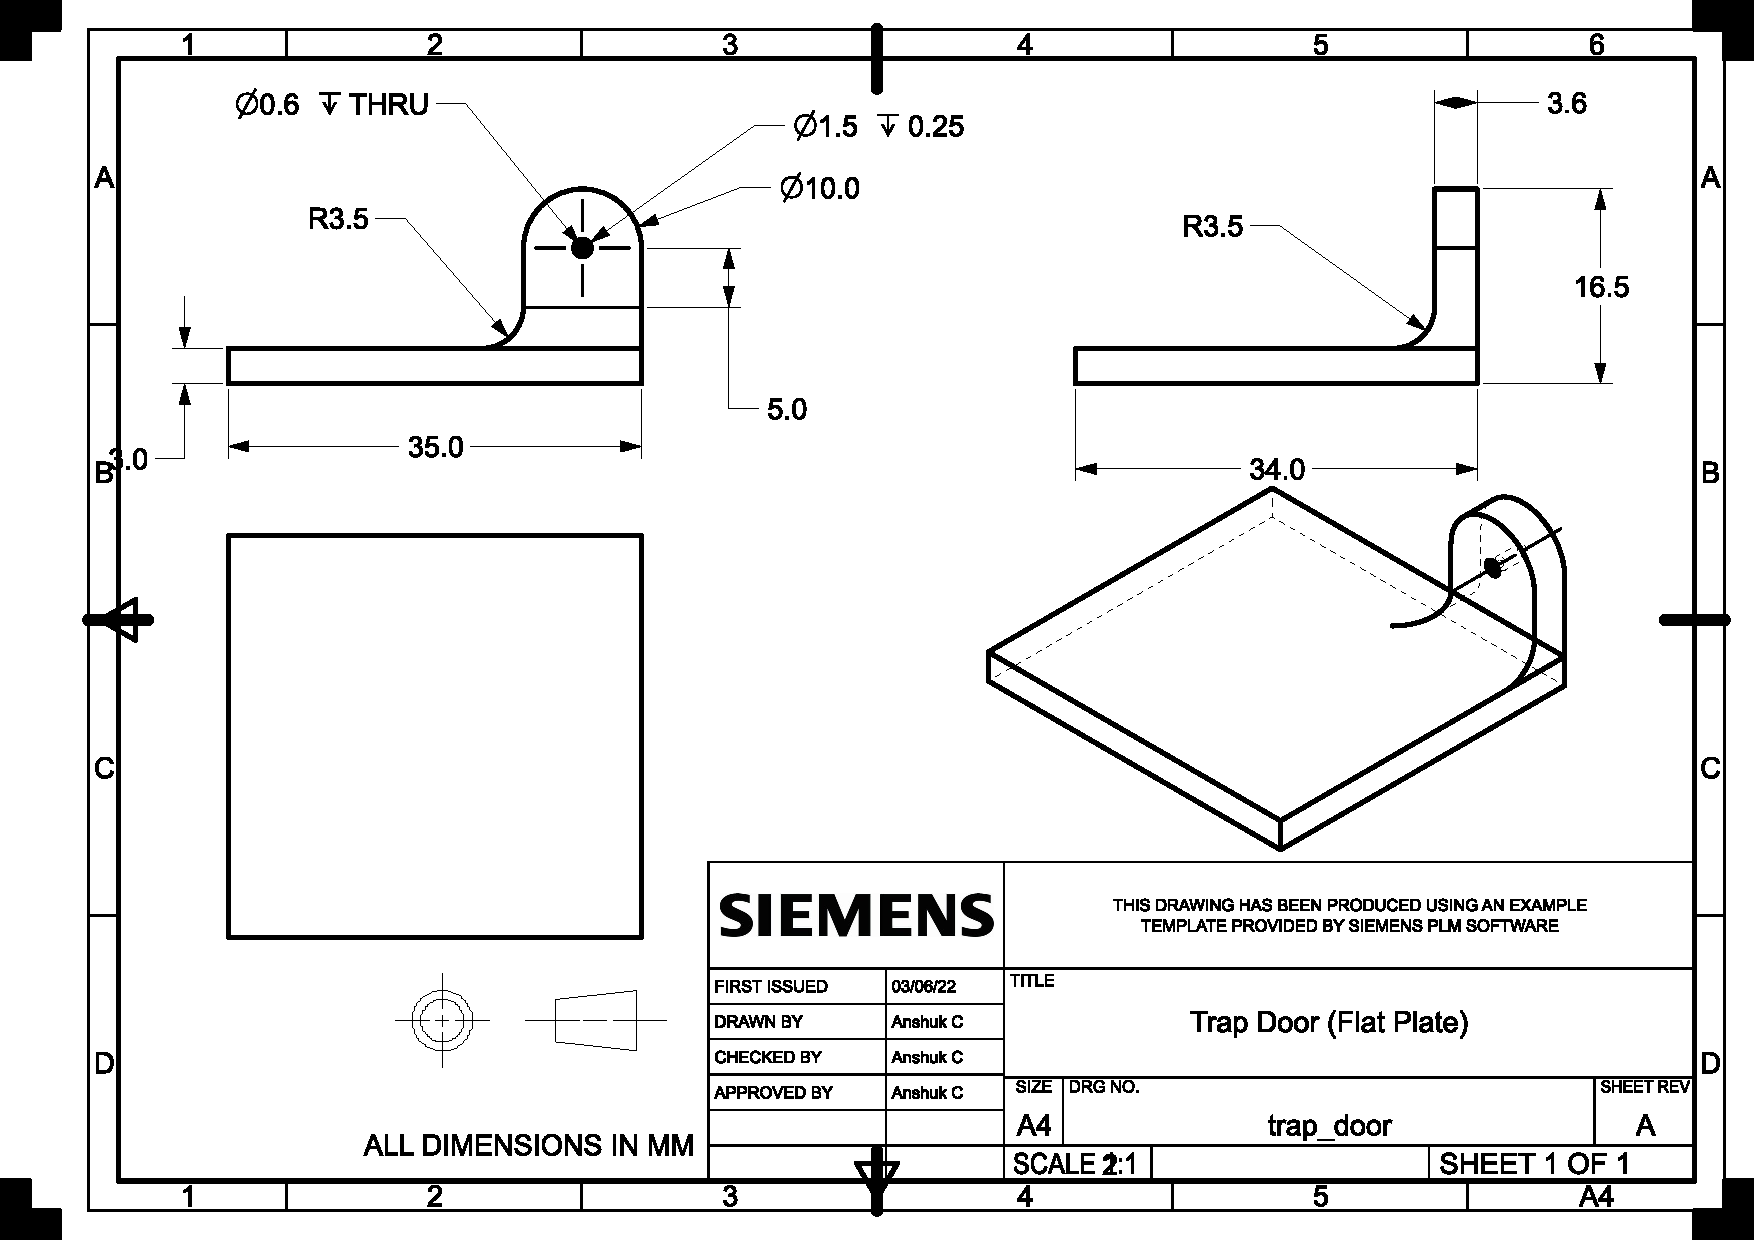
\includepdf[pages=-,angle=90]{homeworks/homework4/report/Figure/vial_plate_drawing.pdf}
    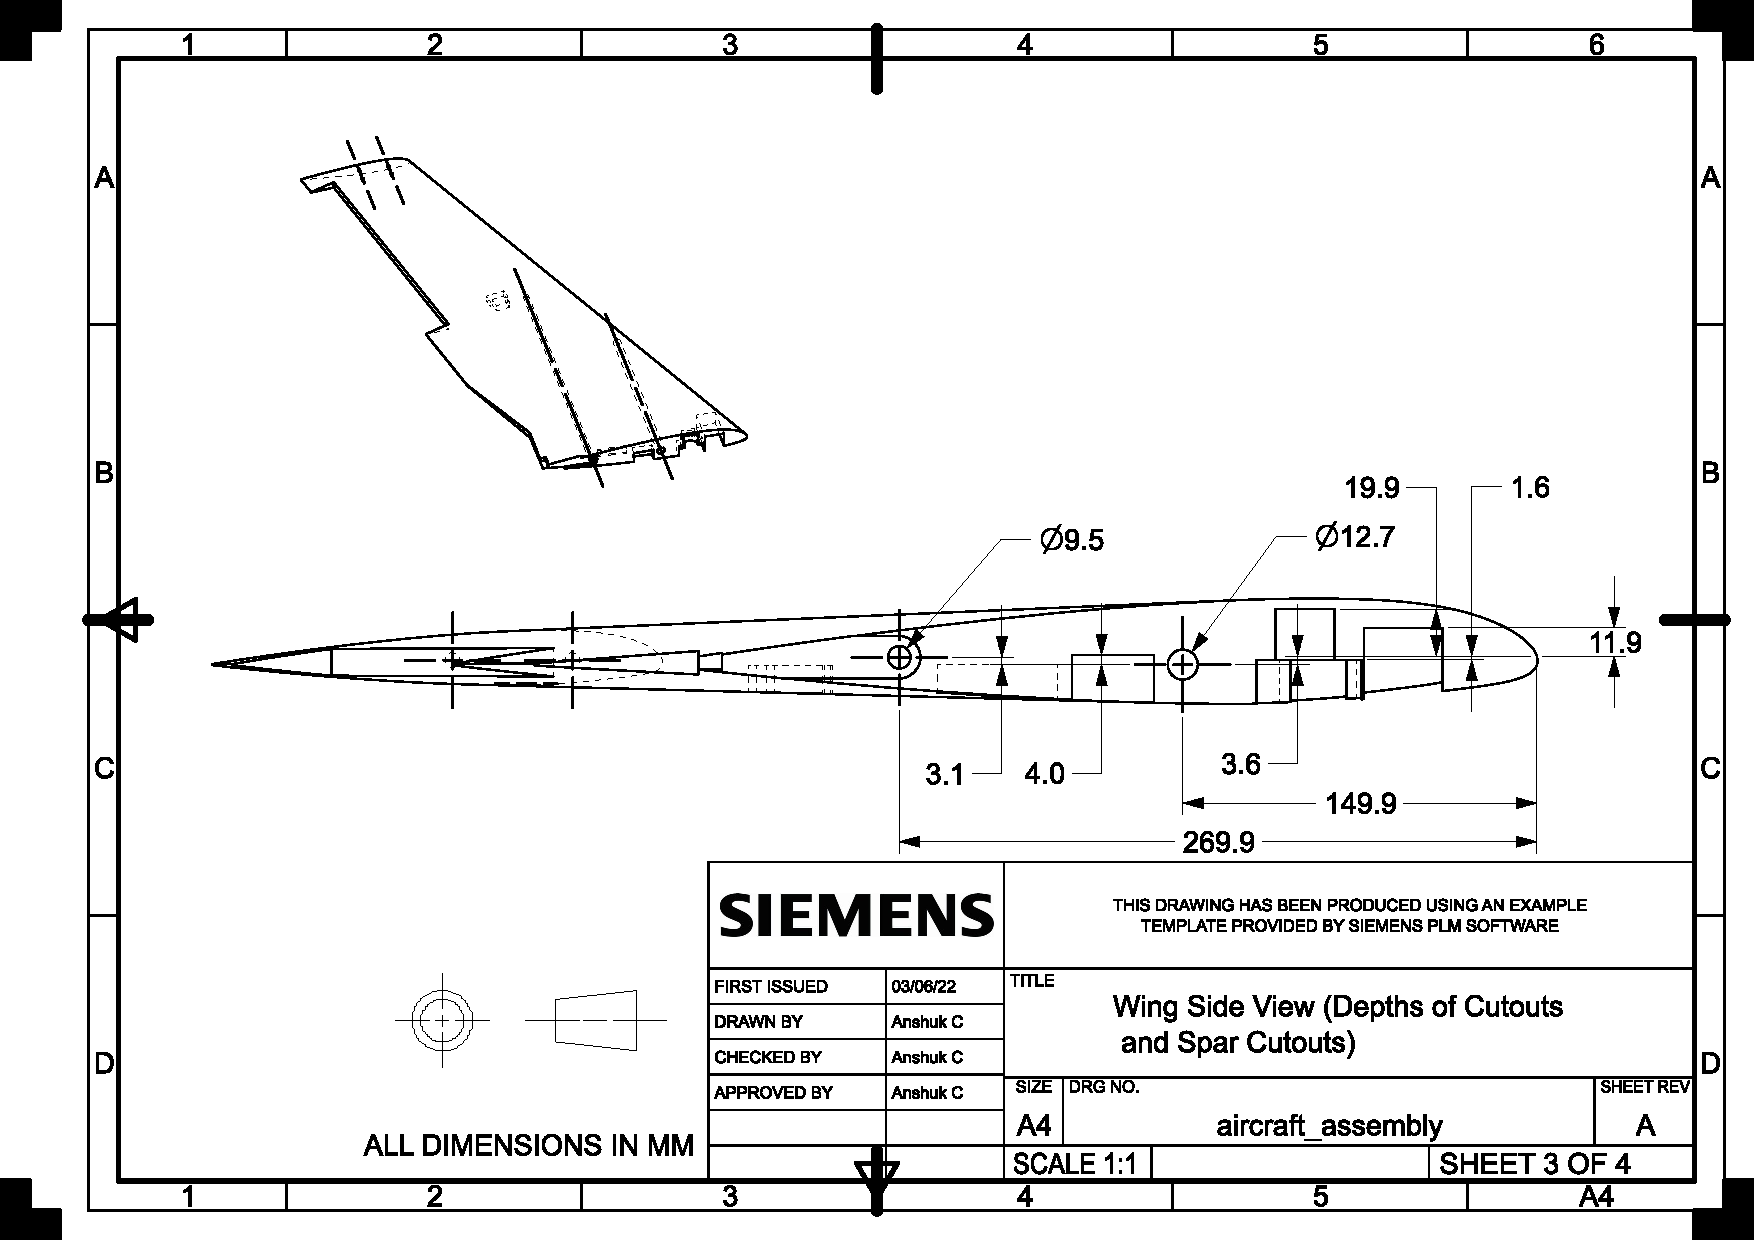
\includepdf[pages=-,angle=90]{homeworks/homework4/report/Figure/wing_depths_spar_cutouts.pdf}
    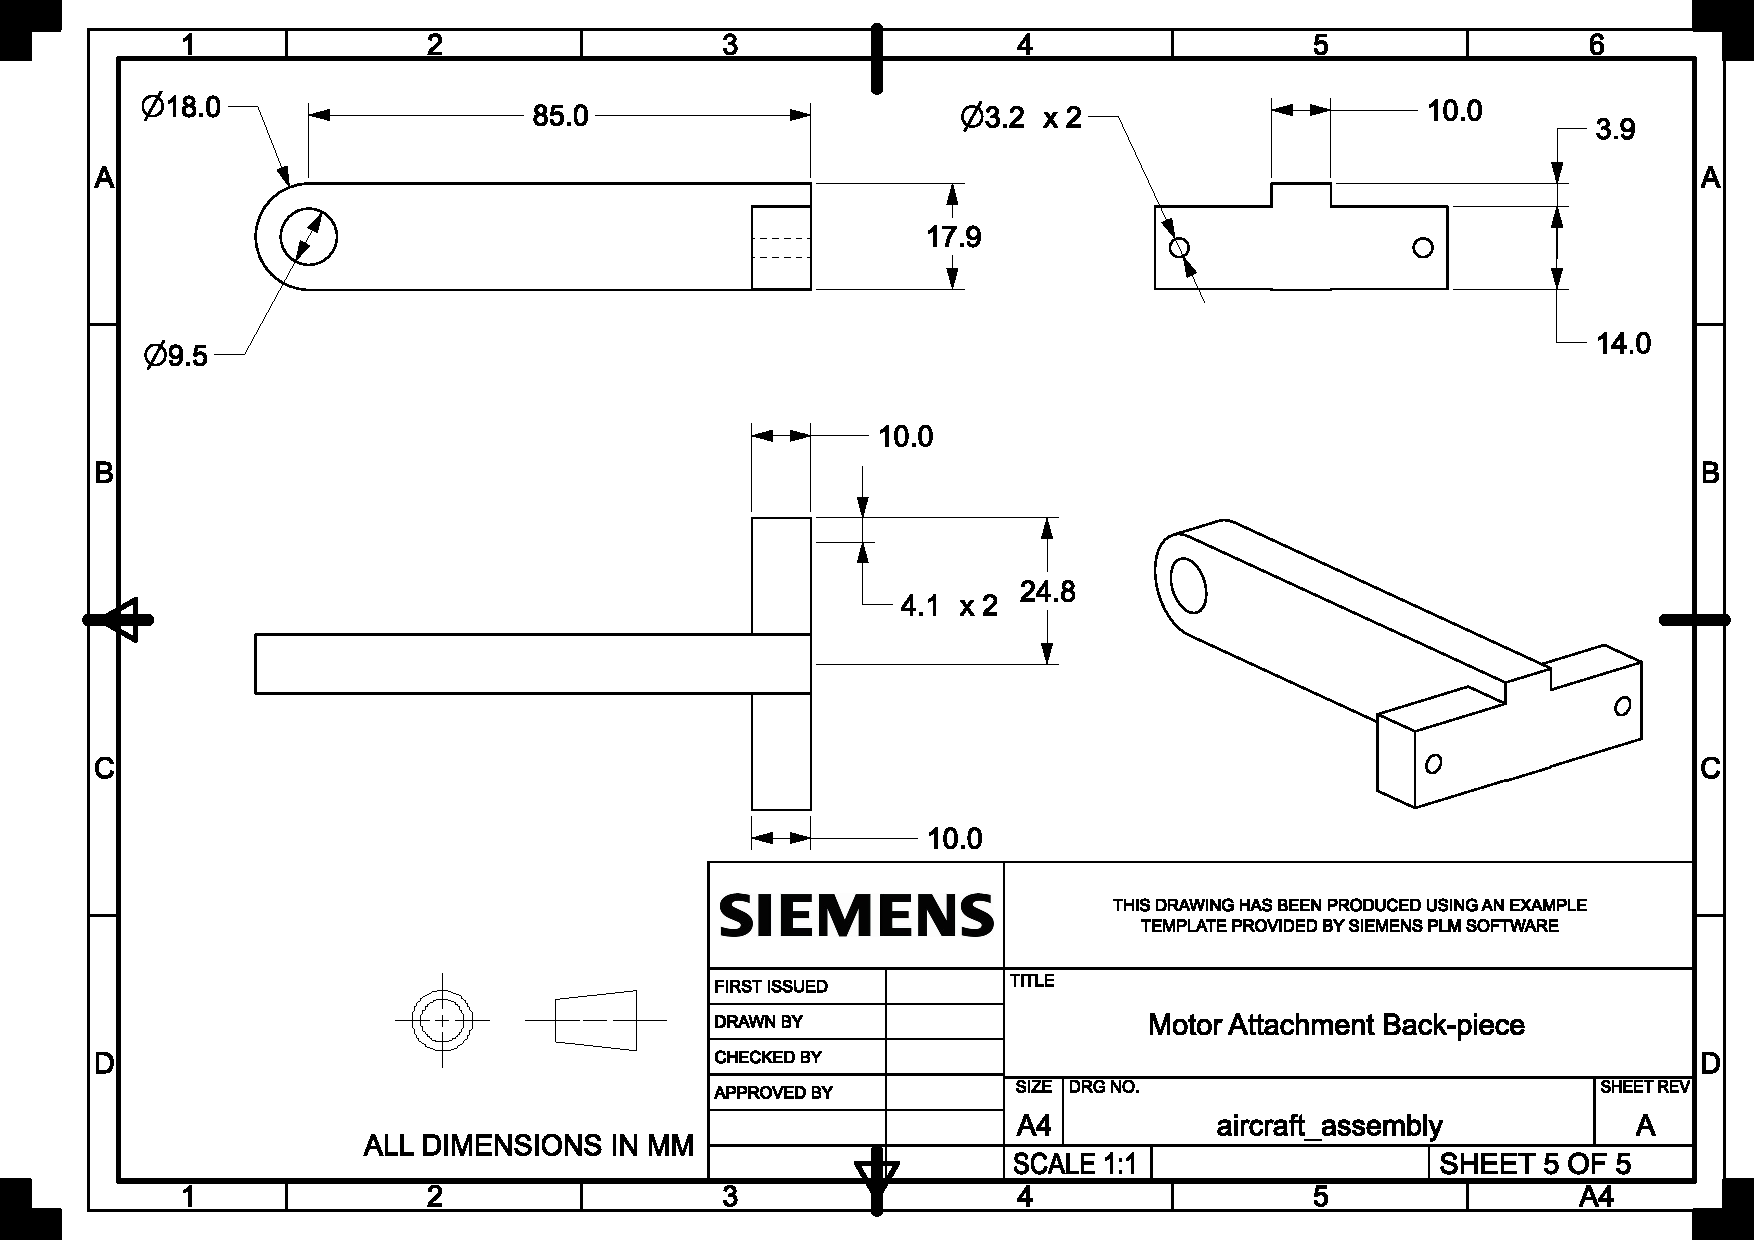
\includepdf[pages=-,angle=90]{homeworks/homework4/report/Figure/motor_holder.pdf}
    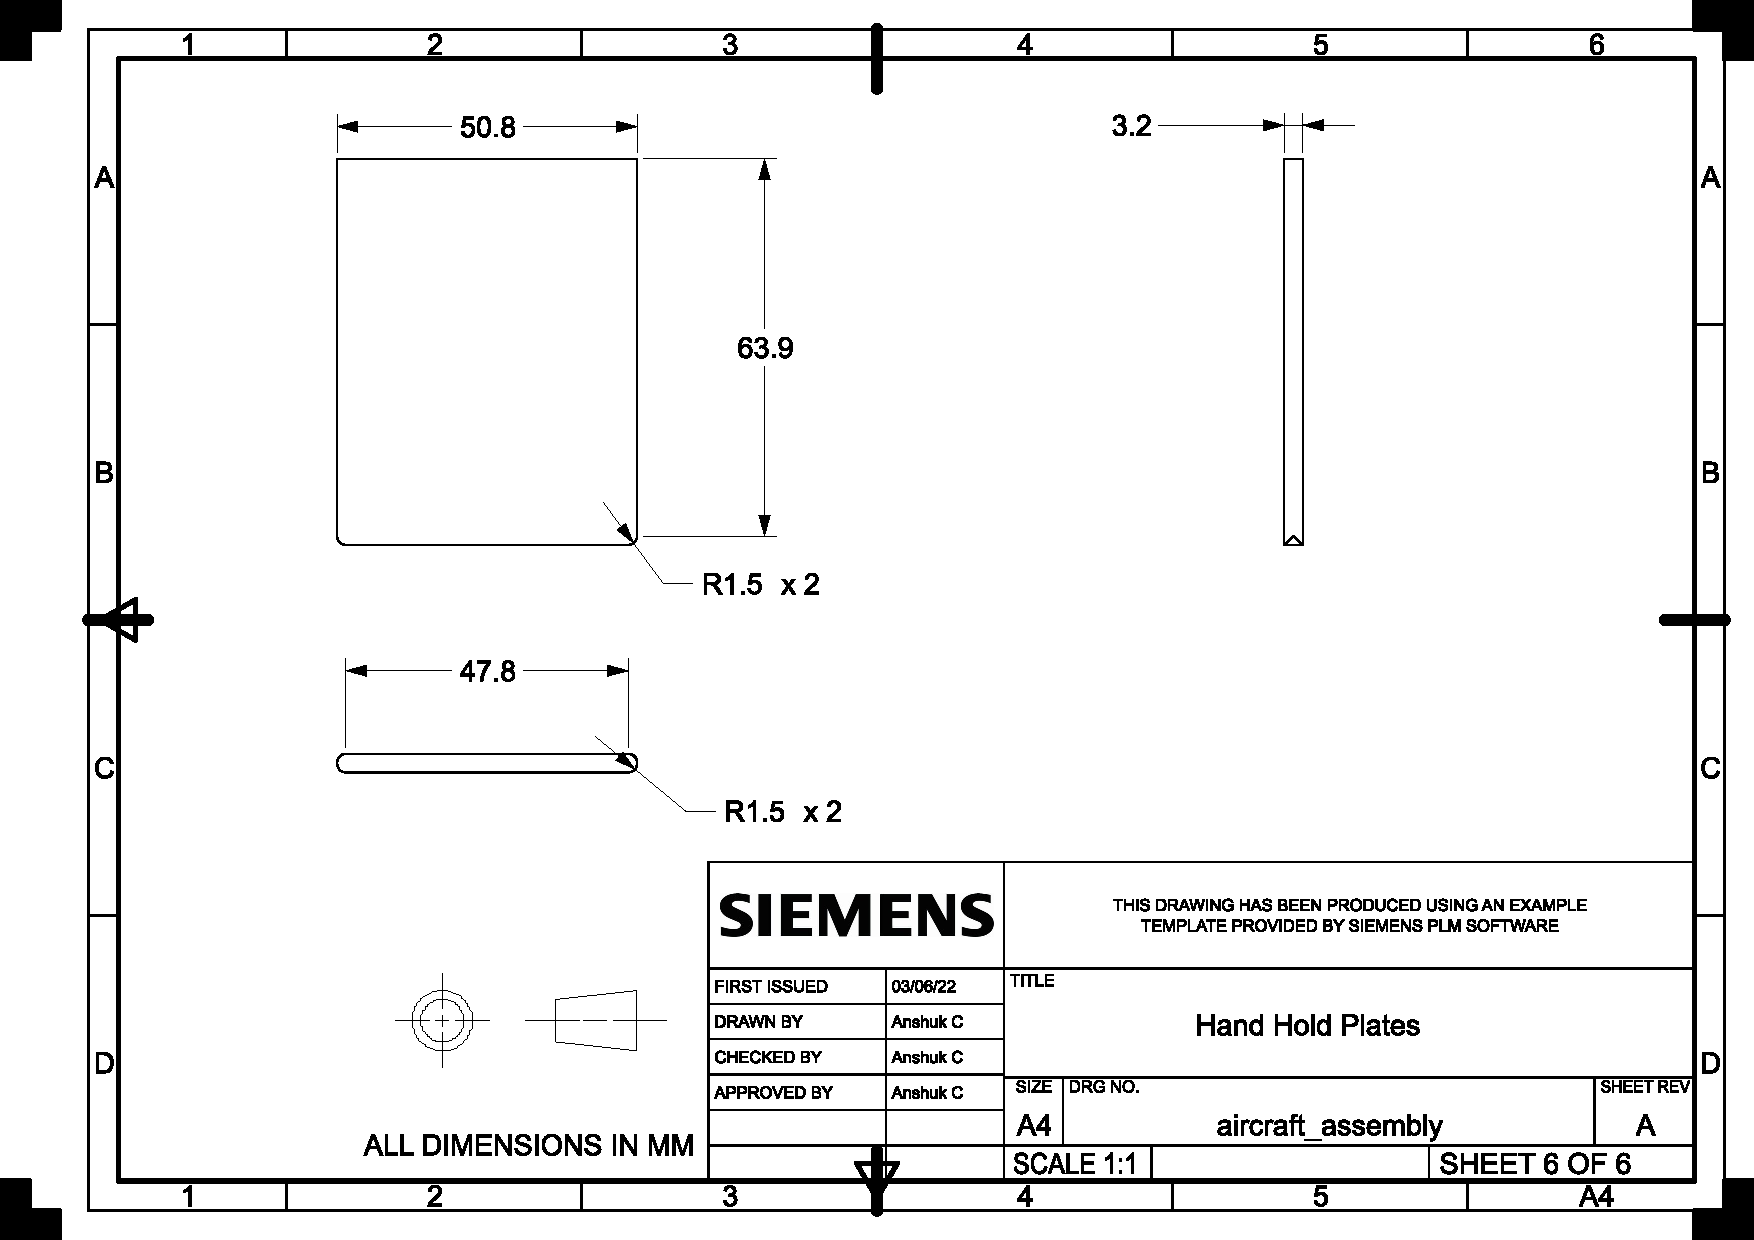
\includepdf[pages=-,angle=90]{homeworks/homework4/report/Figure/hand_holds.pdf}
    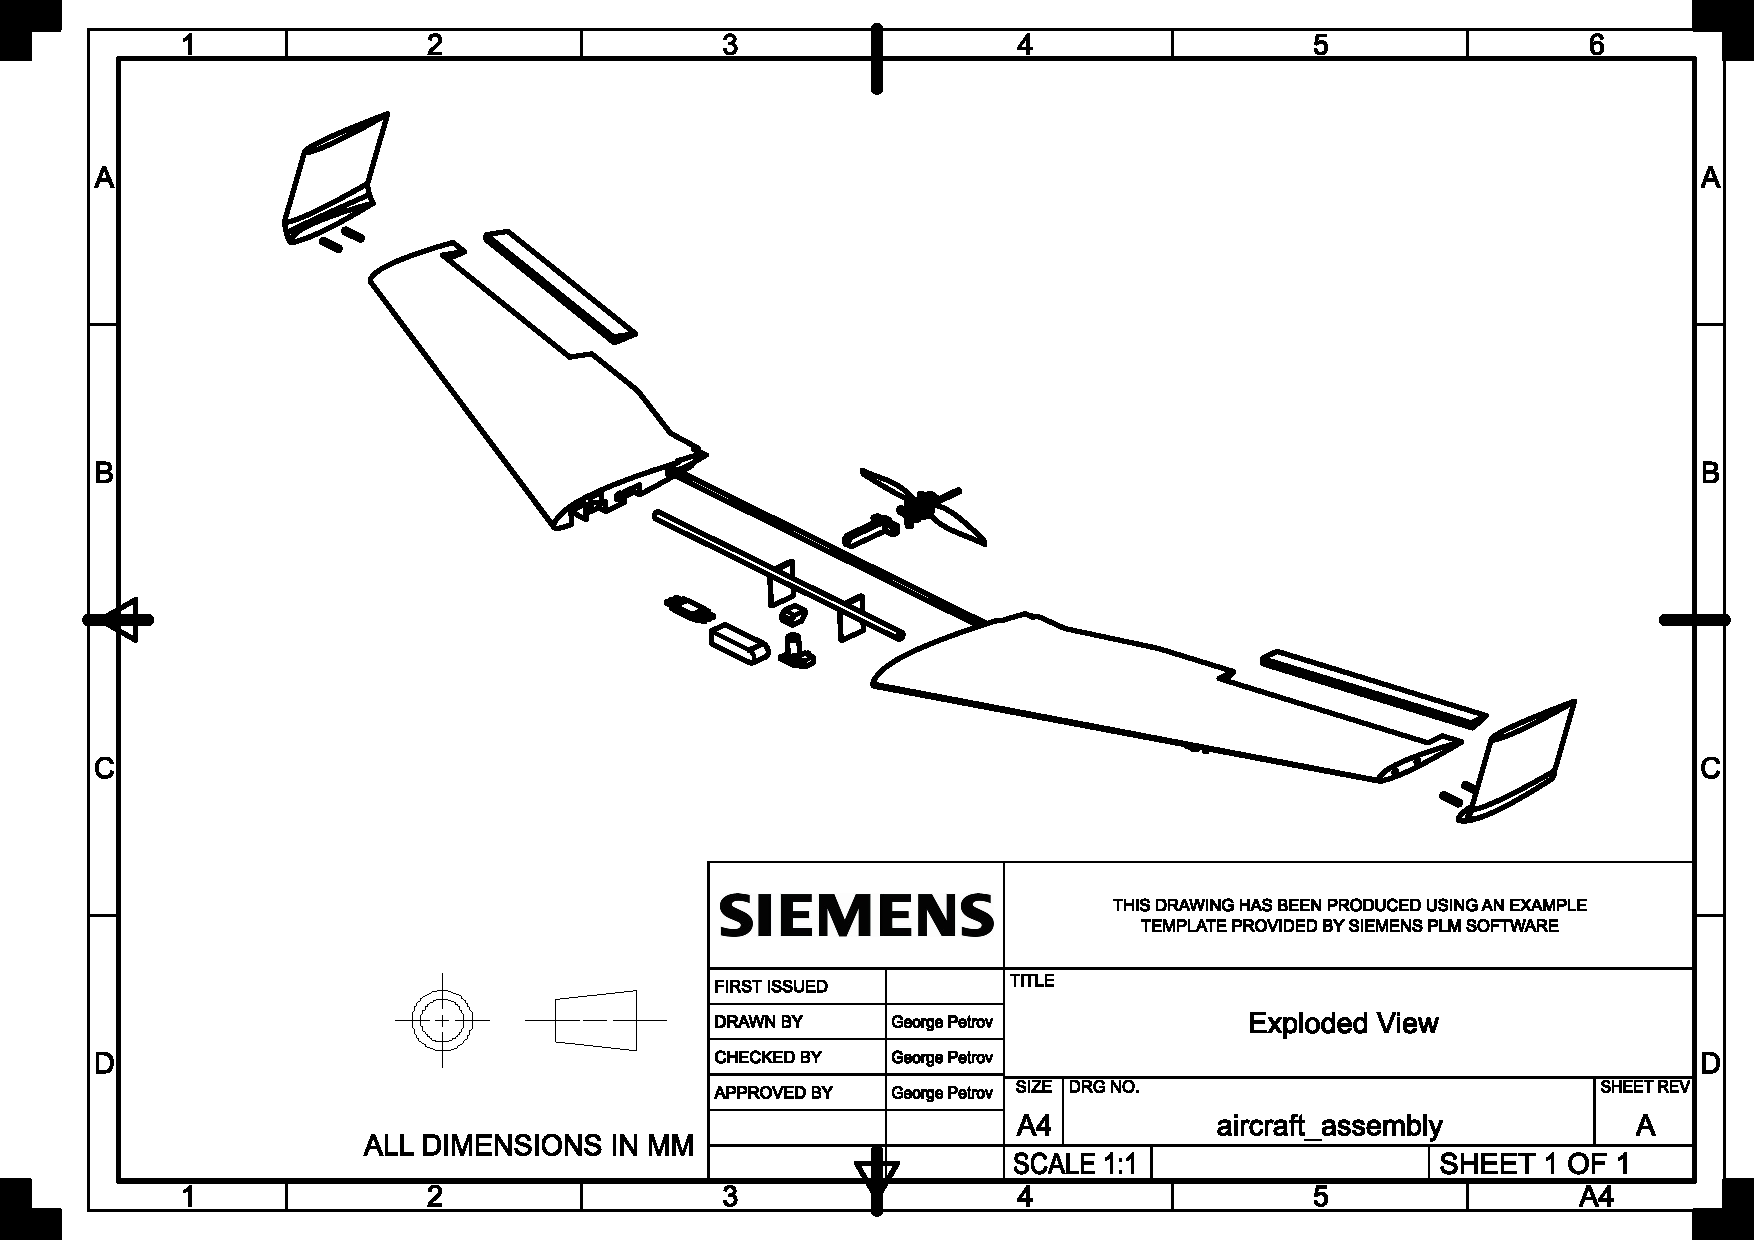
\includepdf[pages=-,angle=90]{homeworks/homework4/report/Figure/gpetrov2_aircraft_assembly_exploded_drawing.pdf}
    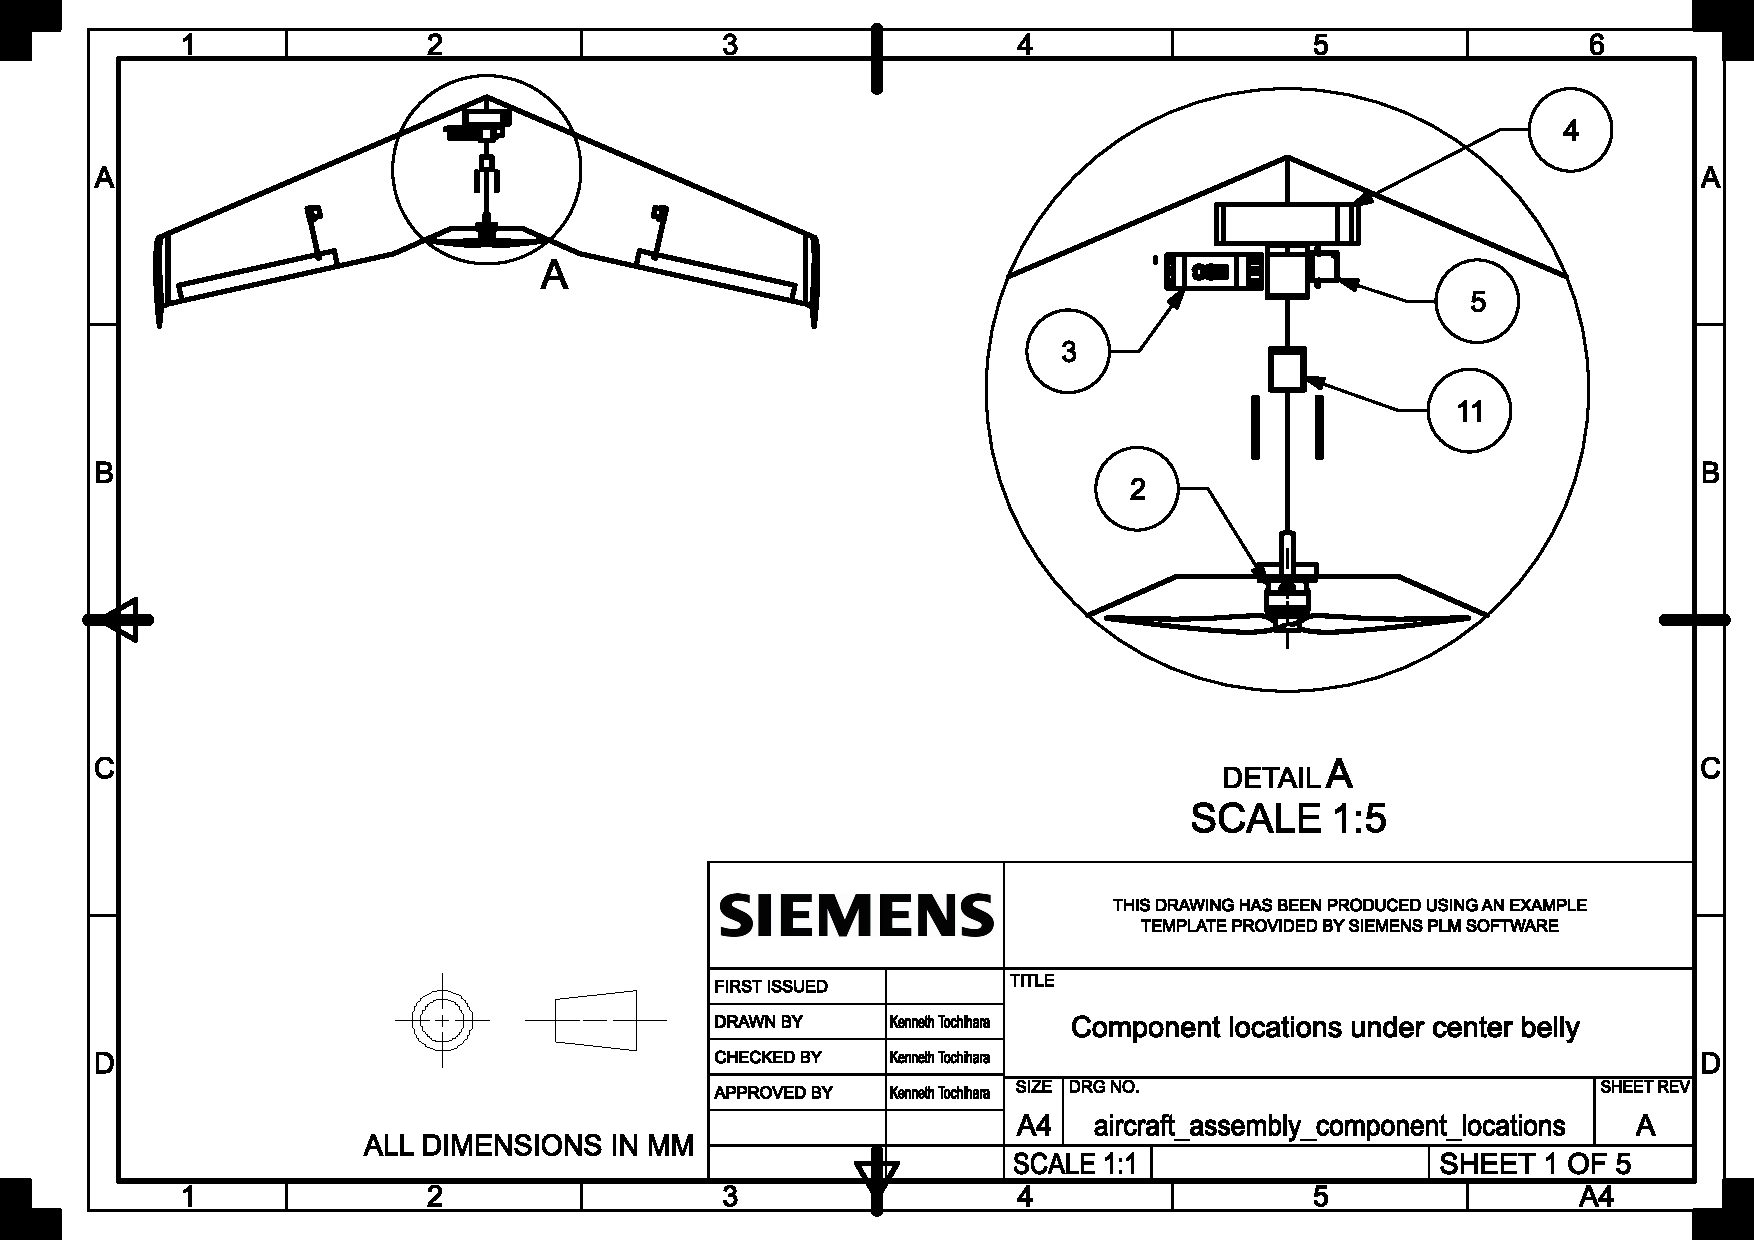
\includepdf[pages=-,angle=90]{homeworks/homework4/report/Figure/ktt3_aircraft_assembly_component_locations.pdf}


\section{Group Member Contributions} \label{apx:contributions}
% Make a table indicating how each group member contributed to the report

    \begin{table}[H]
        \begin{center} 
        \caption{\textbf{Group Member Contributions}}
        \begin{tabular}{ | p{2in} | p{4in}| } 
            \hline
            \textbf{Group Member} & \textbf{Contribution} \\  \hline
            Anshuk Chigullapalli & Designed vial release mechanism, assisted with cutouts, generated engineering drawings for fabricated components and full assembly\\ \hline
            Max Kaiser & Created the XFLR5 model of the UAV, with and without winglets. Completed sections 5,6 and 7 of the report. \\ \hline
            George Petrov & Designed wing, designed cutouts, integrated components, generated exploded views, sample calculations \\ \hline
            Kenneth Tochihara & Designed elevon actuator, designed cutouts, integrated components, generated equipment locations, managed repository \\ \hline
            Jeffery Zhou & \\ \hline
        \end{tabular}
        \end{center}
    \end{table}
    
\end{enumerate}

\end{document}